% ---------------------------------------------------------------------------
%  English research paper
%  Libertinus Serif / Math (bundled), small-caps headings, numbered citations
%  via biblatex + biber. The study, numbers and authors are fictional examples:
%  replace them with your own and keep the structure.
% ---------------------------------------------------------------------------
\documentclass[11pt]{article}

\usepackage[a4paper,textwidth=15cm,top=2.6cm,bottom=3cm,headsep=1cm]{geometry}
\usepackage{fontspec}
\usepackage{unicode-math}
\setmainfont{LibertinusSerif}[
  Extension=.otf, UprightFont=*-Regular, ItalicFont=*-Italic,
  BoldFont=*-Semibold, BoldItalicFont=*-SemiboldItalic]
\setsansfont{LibertinusSans}[
  Extension=.otf, UprightFont=*-Regular, ItalicFont=*-Italic, BoldFont=*-Bold]
\setmathfont{LibertinusMath-Regular.otf}
\setmonofont{SourceCodePro}[Extension=.otf, UprightFont=*-Regular, BoldFont=*-Semibold, Scale=MatchLowercase]

\usepackage{microtype}
\usepackage{xcolor}
\usepackage{graphicx}
\usepackage{booktabs}
\usepackage{caption}
\usepackage{enumitem}
\usepackage{titlesec}
\usepackage{fancyhdr}
\usepackage{pgfplots}
\pgfplotsset{compat=1.18}
\usepackage[backend=biber,style=numeric-comp,sorting=none,maxbibnames=4]{biblatex}
\addbibresource{refs.bib}
\usepackage{hyperref}
\usepackage[capitalise,noabbrev]{cleveref}

% Palette: a dark neutral for structure and a single green accent. Use the accent sparingly.
\definecolor{ink}{HTML}{1F3A33}
\definecolor{accent}{HTML}{2F7D63}
\definecolor{mist}{HTML}{75837E}
\hypersetup{colorlinks, linkcolor=ink, citecolor=accent, urlcolor=accent}

\captionsetup{font=small, labelfont={sc,color=ink}, labelsep=period, width=.92\linewidth}
\setlist{itemsep=2pt, topsep=4pt}

\titleformat{\section}{\large\scshape\color{ink}}{\thesection}{1em}{\lowercase}
\titleformat{\subsection}{\normalsize\itshape}{\thesubsection}{1em}{}
\titlespacing*{\section}{0pt}{2.2ex plus .5ex}{1.2ex}

\pagestyle{fancy}
\fancyhf{}
\renewcommand{\headrulewidth}{0pt}
\fancyhead[C]{\footnotesize\scshape\color{mist}the quiet page}
\fancyfoot[C]{\footnotesize\thepage}

\newtheorem{hypothesis}{Hypothesis}

\begin{document}

% ---------------------------------------------------------------- title block
\thispagestyle{empty}
\begin{center}
  {\color{accent}\footnotesize\scshape research article}\par\vspace{10pt}
  {\LARGE\bfseries The Quiet Page:\par}\vspace{4pt}
  {\Large Line Length, Leading, and the Speed of Reading on Screens\par}
  \vspace{16pt}
  {\scshape Mira Okafor}\textsuperscript{1}\quad\textperiodcentered\quad
  {\scshape Tomás Ilves}\textsuperscript{2}\quad\textperiodcentered\quad
  {\scshape Hana Sato}\textsuperscript{1}\par
  \vspace{6pt}
  {\footnotesize\itshape
    \textsuperscript{1}Reading Lab, Northfield University \qquad
    \textsuperscript{2}Institute for Visual Communication\par
    \textup{\texttt{mira.okafor@northfield.edu}}\par}
  \vspace{14pt}
  {\color{ink}\rule{3cm}{.6pt}}
\end{center}

\begin{quote}
  \small
  \noindent\textsc{\color{ink}Abstract.}\enspace
  Typographers have long recommended 45--75 characters per line, yet most of
  that advice was formed on paper. We asked 312 adults to read 24 short essays on
  screens while we varied line length and line spacing independently. Reading
  speed peaked at about 66 characters per line and fell off sharply beyond 90;
  generous leading recovered most of the loss at long measures, but none of it
  at short ones. Comprehension stayed flat across conditions, which suggests that
  readers trade effort, not understanding. We release the essays, the stimuli and
  the analysis code.

  \vspace{6pt}\noindent\textsc{\color{ink}Keywords.}\enspace
  typography, legibility, reading speed, line length, screen reading
\end{quote}
\vspace{6pt}

% ---------------------------------------------------------------- body
\section{Introduction}

Every reader has met a page that feels \emph{tiring} before a single word has
been read: lines that run edge to edge on a wide monitor, or a narrow column that
breaks a sentence every few words. Bringhurst's rule of thumb---45 to 75
characters, with 66 as the ideal~\cite{bringhurst2004}---descends from studies of
printed matter going back almost a century~\cite{tinker1929}. Screens differ from
paper in resolution, distance and, above all, in how readily the reader can
change the layout.

We revisit the question with three aims:
\begin{enumerate}[label=(\roman*)]
  \item measure reading speed and comprehension across line lengths that are
        common in today's interfaces;
  \item separate the effect of line length from that of line spacing, which are
        usually changed together;
  \item publish materials that others can rerun on their own screens.
\end{enumerate}

\begin{hypothesis}
  \label{hyp:peak}
  Reading speed is an inverted U in line length, with a peak inside the
  45--75 character band.
\end{hypothesis}

\begin{hypothesis}
  \label{hyp:leading}
  Extra line spacing helps more at long line lengths, where the eye must find
  the start of the next line after a long return sweep~\cite{dyson2004}.
\end{hypothesis}

\section{Method}

\subsection{Participants and materials}
We recruited 312 adults (median age 31) who read English daily. Each read 24
essays of about 450 words, set in the same typeface and size, under a
$6 \times 4$ within-subject design: six line lengths from 35 to 115 characters
and four line spacings from $1.0$ to $1.6$ times the font size. Paragraphs were
justified with the Knuth--Plass algorithm~\cite{knuth1981} so that word spacing
stayed even across conditions.

\subsection{Measures}
Reading speed is words per minute on the first read. After each essay,
readers answered four multiple-choice questions. We fit a mixed model
\begin{equation}
  \label{eq:model}
  \log \mathrm{wpm}_{ij} = \beta_0 + f(L_j) + \beta_s\, S_j + \beta_{Ls}\, L_j S_j
    + u_i + v_{e(j)} + \varepsilon_{ij},
\end{equation}
where $L_j$ is line length, $S_j$ is spacing, $f$ is a restricted cubic spline,
and $u_i$ and $v_{e(j)}$ are random intercepts for reader and essay.

\section{Results}

\Cref{fig:speed} shows the central finding: speed rises until about 66
characters and declines past 90, supporting \cref{hyp:peak}. Wider spacing lifts
the curve only on the right-hand side, as \cref{hyp:leading} predicted.
\Cref{tab:results} reports the same pattern as numbers.

\begin{figure}[t]
  \centering
  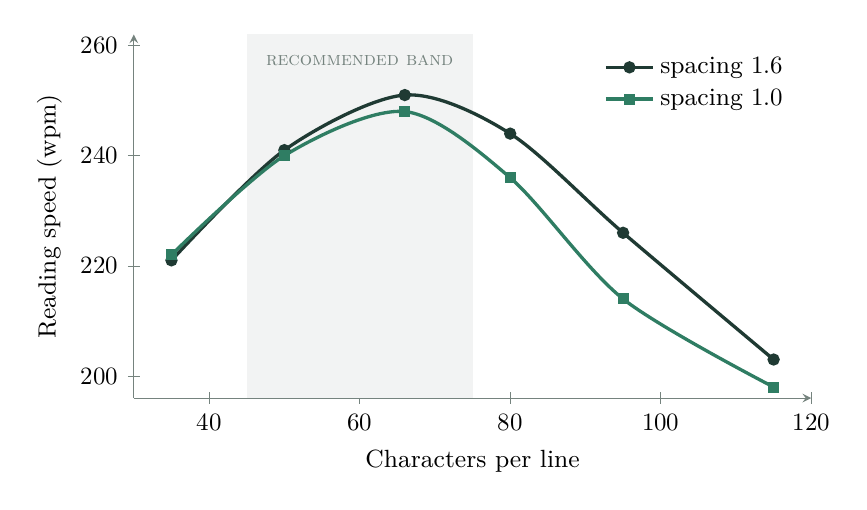
\begin{tikzpicture}
    \begin{axis}[
      width=.84\linewidth, height=6.2cm,
      xlabel={Characters per line}, ylabel={Reading speed (wpm)},
      xmin=30, xmax=120, ymin=196, ymax=262,
      axis lines=left, tick style={mist}, axis line style={mist},
      tick label style={font=\small}, label style={font=\small},
      legend style={draw=none, font=\small, at={(0.98,0.97)}, anchor=north east},
      every axis plot/.append style={very thick, smooth},
    ]
      \fill[ink!6] (axis cs:45,196) rectangle (axis cs:75,262);
      \node[font=\scriptsize\scshape, text=mist, anchor=north] at (axis cs:60,260) {recommended band};
      \addplot[ink, mark=*, mark size=1.6pt] coordinates
        {(35,221) (50,241) (66,251) (80,244) (95,226) (115,203)};
      \addlegendentry{spacing $1.6$}
      \addplot[accent, mark=square*, mark size=1.4pt] coordinates
        {(35,222) (50,240) (66,248) (80,236) (95,214) (115,198)};
      \addlegendentry{spacing $1.0$}
    \end{axis}
  \end{tikzpicture}
  \caption{Mean reading speed by line length. Generous spacing helps long lines
    but cannot rescue them; short lines gain nothing.}
  \label{fig:speed}
\end{figure}

\begin{table}[t]
  \centering
  \caption{Reading speed and comprehension at three representative measures
    (spacing $1.3$). Speeds are means $\pm$ standard error.}
  \label{tab:results}
  \begin{tabular}{@{}l r r r@{}}
    \toprule
    Characters per line & Speed (wpm)              & Comprehension & Preferred \\
    \midrule
    35                  & $221 \pm 3$              & 0.86          & 9\%       \\
    66                  & $\mathbf{250} \pm 3$     & 0.87          & 64\%      \\
    105                 & $209 \pm 4$              & 0.85          & 27\%      \\
    \bottomrule
  \end{tabular}
\end{table}

\section{Discussion}

Our readers did not understand less on long lines; they worked harder to
understand the same. The cost is paid in time and, we suspect, in fatigue over
longer sessions. For designers the practical rule is simple: cap the measure
first, and add leading only when a long measure cannot be avoided.

\paragraph{Limitations.} All essays were expository English prose. Code,
tables and languages without word spaces may behave differently.

\section{Conclusion}

A century-old rule survives the move to screens almost unchanged. The page that
reads fastest is still the quiet one: a modest measure, even spacing, and
nothing that asks the eye to search for its place.

\paragraph{Data availability.} Essays, stimuli and analysis code are available at
\url{https://example.org/quiet-page}.

\printbibliography

\end{document}
